%! TeX program = lualatex
\documentclass[a4paper]{article} 

% packages
\usepackage{microtype}      % Slightly tweak font spacing for aesthetics
\usepackage[english]{babel} % Language hyphenation and typographical rules
\usepackage[final, colorlinks = true, urlcolor = black, linkcolor = black, citecolor = black]{hyperref} 
\newcommand{\secref}[1]{\textbf{§\ref{#1}~\nameref{#1}}}
\usepackage{changepage}     % adjust margins on the fly
\usepackage{multicol}

\usepackage{amsmath}
\usepackage{amssymb}
\usepackage{amsfonts}

\usepackage[backend=biber, style=numeric, date=iso, urldate=iso]{biblatex}
\addbibresource{references.bib}
\DeclareFieldFormat{urldate}{Accessed on: #1}

\usepackage{fontspec}
\setmainfont{EB Garamond}
\setmonofont[Scale=MatchLowercase]{Deja Vu Sans Mono}

\usepackage{minted}
\usemintedstyle{algol_nu}
\usepackage{xcolor}

\usepackage{pgfplots}
\pgfplotsset{width=\textwidth,compat=1.9}

\usepackage{caption}
\newenvironment{code}{\captionsetup{type=listing}}{}
\captionsetup[listing]{skip=0pt}
\setlength{\abovecaptionskip}{5pt}
\setlength{\belowcaptionskip}{5pt}

\usepackage[yyyymmdd]{datetime}
\renewcommand{\dateseparator}{--}

\usepackage{tikz}
\usetikzlibrary{trees}

\usepackage{titlesec}
% \titleformat{\section}{\LARGE\bfseries}{}{}{}[\titlerule]
% \titleformat{\subsection}{\Large\bfseries}{}{0em}{}
% \titlespacing{\subsection}{0em}{-0.7em}{0em}
%
% \titleformat{\subsubsection}{\large\bfseries}{}{0em}{$\bullet$ }
% \titlespacing{\subsubsection}{1em}{-0.7em}{0em}

\addtolength{\hoffset}{-2.25cm}
\addtolength{\textwidth}{4.5cm}
\addtolength{\voffset}{-3.25cm}
\addtolength{\textheight}{5cm}
\setlength{\parskip}{0pt}
\setlength{\parindent}{0in}

\begin{document}
\hrule \medskip
\begin{minipage}{0.295\textwidth} 
    \vfill
    \raggedright
    \footnotesize 
    \begin{tabular}{@{}l l} % Define a two-column table with left alignment
        Name: & Andrew Hayes \\
        Student ID: & 21321503 \\
        Programme: & 4BCT \\
    \end{tabular}
    \vfill
\end{minipage}
\begin{minipage}{0.4\textwidth} 
    \centering 
    \LARGE 
    \vfill
    \textsc{ct4101}
    \vfill
\end{minipage}
\begin{minipage}{0.295\textwidth} 
    \raggedleft
    \vfill
    \today
    \vfill
\end{minipage}
\smallskip
\hrule 
\begin{center}
    \normalsize
    Assignment 2: Regression Using Scikit-Learn
\end{center}
\hrule

\section{Description of Algorithms}
\subsection{Algorithm 1: Random Forest}
\textbf{Random forest} is a supervised machine learning algorithm used for classification and regression tasks.
It builds upon the \textbf{decision tree} algorithm by constructing a collection of decision trees, where each tree is trained independently on random subsets of the data.
These trees are then aggregated to make the final prediction. 
An implementation of this algorithm for regression is provided in scikit-learn as \mintinline{python}{sklearn.ensemble.RandomForestRegressor} \supercite{scikit_randomforestregressor}. 
\\\\
To overcome the problems of decision trees being unstable and causing overfitting, the random forest algorithm combines many randomly-generated decision trees into a single forest to improve accuracy, reduce overfitting, \& reduce variance.
Each tree is built independently on a different random subset of the training data and features, which helps reduce variance and overfitting. 
The final prediction is obtained by averaging the predictions of each individual tree (for regression tasks) or by majority voting (for classification tasks).
The accuracy of the model in random forests is improved through \textbf{bagging}, a technique that averages predictions over a large number of independently trained trees to reduce variance and prevent overfitting.
\\\\
In \mintinline{python}{RandomForestRegressor}, the trees are constructed as follows:
\begin{enumerate}
    \item   The algorithm generates multiple bootstrap samples by randomly selecting subsets of the training data with replacement.
            These subsets are used to train individual decision trees.
            Selecting the samples with replacement allows the generated trees to overlap, which helps to reduce variance and overfitting.

    \item   Each node is split to partition the data, decided by a random subset of the features.
            The split that causes the greatest reduction in error according to the mean squared error algorithm is chosen.
            This process is repeated for every node starting at the root node until there are no splits left to be made.

    \item   The final prediction is made by averaging the predictions of all the individual trees in the forest (for regression tasks).
\end{enumerate}

I chose the random forest regressor because it is robust to overfitting, handles high-dimensional datasets well, and offers strong performance without requiring extensive tuning of hyperparameters. 
It is also an interesting comparison to the gradient boosting regressor, as both are ensemble methods that leverage multiple decision trees but with different strategies for combining these trees.

\subsubsection{Hyperparameter 1: \mintinline{python}{n_estimators}}
The hyperparameter \mintinline{python}{n_estimators} is an \mintinline{python}{int} with a default value of 100, which controls the number of decision trees added to the model \supercite{scikit_randomforestregressor}. 
Increasing the number of estimators generally improves model accuracy and stability, but it may lead to overfitting if too many trees are added. 
Thus, there is a trade-off between performance and computational cost, as more estimators require more training time and resources.

\subsubsection{Hyperparameter 2: \mintinline{python}{max_depth}}
The hyperparameter \mintinline{python}{max_depth} is an \mintinline{python}{int} with a default value of \mintinline{python}{None}, controlling the maximum depth of each tree in the ensemble \supercite{scikit_gradientboostingregressor}. 
By limiting the depth, the algorithm helps prevent overfitting, as shallower trees capture more general patterns in the data.
High \mintinline{python}{max_depth} values allow trees to capture complex patterns, but can lead to overfitting and reduced generalisation on unseen data. 
In contrast, lower \mintinline{python}{max_depth} values create simpler trees that focus on the most important features and relationships, which can enhance generalisation but may result in underfitting if the model fails to capture necessary data complexity.

\subsection{Algorithm 2: Gradient Boosting}\label{sec:alg2desc}
\textbf{Gradient boosting} is a supervised machine learning algorithm that can be used for both classification \& regression tasks. 
It builds upon the \textbf{decision tree} algorithm by combining multiple decision trees sequentially, with each new tree trained to correct the errors of the previous ones. 
This sequential training process is distinct from that of \textbf{random forests}, which aggregates many trees independently trained on random subsets of the data.
An implementation of this algorithm for regression is provided in scikit-learn as \mintinline{python}{sklearn.ensemble.GradientBoostingRegressor} \supercite{scikit_gradientboostingregressor}. 
While gradient boosting can also be used for classification, I will only refer to its use as a regression algorithm in this assignment, as classification is not relevant to the specific task at hand.
\\\\
While both random forest and gradient boosting use multiple decision trees, they differ fundamentally in how they build and combine these trees:
\begin{itemize}
    \item   In \textbf{Random Forest}, trees are built independently on random subsets of data and features, which helps reduce variance and improves generalisation. 
    The final prediction is obtained by averaging the outputs of each tree (for regression tasks) or by majority voting (for classification tasks).

    \item   In \textbf{Gradient Boosting}, trees are built sequentially, with each new tree trained to correct the errors of the previous ones. 
    This iterative process focuses on reducing bias, as each tree addresses the residual errors from prior iterations.
    The final prediction is obtained by summing the predictions of each tree, where later trees contribute to refining the overall model.
    This general process of creating new models to sequentially correct the errors of previous iterations is called \textbf{boosting}: these iterative models are called \textit{weak learners} (in this context, the decision trees are the weak learners) and are combined to form what is (hopefully) a \textit{strong learner}.
    These weak learners are typically only somewhat more accurate than random guessing, and are often very shallow trees, but when combined can produce very accurate results. 
\end{itemize}

The accuracy of the weak learners is assessed with a \textbf{loss function} which quantifies the error in the model.
While \mintinline{python}{GradientBoostingRegressor} provides different options for the loss function used, the default is \mintinline{python}{loss = 'squared_error'} or Mean Squared Error, which is a domain-specific measure of error given by:
\[
    \text{MSE} = \frac{ \sum^n_{i=1} ( t_i - \mathbb{M}(d_i) )^2 }{ n }
\]
where $\mathbb{M}(d_1) \dots \mathbb{M}(d_n)$ is a set of $n$ values predicted by the model and $t_1 \dots t_n$ is a set of labels. \supercite{glavo}
\\\\
In \mintinline{python}{GradientBoostingRegressor}, the trees are generated as follows:
\begin{enumerate}
    \item   The algorithm initializes the model with a constant value, which serves as the baseline prediction for all instances.

    \item   At each iteration, the algorithm computes the negative gradient of the loss function with respect to the current model's predictions. 
            This gradient indicates the direction in which to adjust the predictions to minimize the loss.

    \item   A decision tree is then fitted to the negative gradients (i.e., the errors) from the previous iteration, where each tree is constrained in complexity (often by limiting the depth) to avoid overfitting.

    \item   The predictions from this new tree are scaled by a learning rate and added to the ensemble's predictions to update the model.
\end{enumerate}

I chose the gradient boosting regressor because it is effective for complex and non-linear datasets, provides robust performance on diverse types of data, and offers flexibility with numerous hyperparameters for tuning.
It is also an interesting comparison to the random forest regressor, as they both are ensemble methods that use multiple decision trees.

\subsubsection{Hyperparameter 1: \mintinline{python}{n_estimators}}
The hyperparameter \mintinline{python}{n_estimators} is an \mintinline{python}{int} with a default value of 100, which controls the number of boosting stages (i.e., decision trees) added to the model \supercite{scikit_gradientboostingregressor}. 
Increasing the number of estimators generally improves model accuracy and stability, but it may lead to overfitting if too many trees are added. 
Thus, there is a trade-off between performance and computational cost, as more estimators require more training time and resources.

\subsubsection{Hyperparameter 2: \mintinline{python}{max_depth}}
The hyperparameter \mintinline{python}{max_depth} is an \mintinline{python}{int} with a default value of 3, controlling the maximum depth of each tree in the ensemble \supercite{scikit_gradientboostingregressor}. 
By limiting the depth, the algorithm helps prevent overfitting, as shallower trees capture more general patterns in the data.
High \mintinline{python}{max_depth} values allow trees to capture complex patterns, but can lead to overfitting and reduced generalisation on unseen data.
In contrast, lower \mintinline{python}{max_depth} values create simpler trees that focus on the most important features and relationships, which can enhance generalisation but may result in underfitting if the model fails to capture necessary data complexity.

\section{Model Training \& Evaluation}
For both algorithms, I first trained a model with the default hyperparameters using 10-fold cross-variation to get a baseline to which I could compare my results.
To achieve this 10-fold cross-validation, I used the \mintinline{python}{sklearn.model_selection.KFold} and the \mintinline{python}{cross_validate} function which I provided with a seed of \mintinline{python}{random_state=42} to get consistent testing results.
I then tuned my chosen hyperparameters using the \mintinline{python}{GridSearchCV} class.
I performed two grid searches for each algorithm, one with each of my chosen measures of error.

\subsection{Measures of Error}
\subsubsection{Domain-Specific Measure of Error}
I chose \textbf{mean squared error} as my domain-specific measure of error, as it is simple \& intuitive to understand, penalises larger errors more strongly than weaker errors, and because it is the default loss function used in \mintinline{python}{GradientBoosingRegressor}.
Since I did not choose the loss function of \mintinline{python}{GradientBoosingRegressor} as a hyperparameter to tune for this assignment, the \mintinline{python}{GradientBoosingRegressor} will attempt to optimise the MSE of model by default and thus I feel that it would be most appropriate to also use this metric in my own analysis; it doesn't seem effective to tune the model to optimise for one measure of error, and then actually assess the model by using an entirely different measure.
Similarly, \mintinline{python}{RandomForestRegressor} uses MSE to determine the optimal split at a node in the decision trees it creates.
\\\\
The equation by which MSE is defined can be found above in \secref{sec:alg2desc}.

\subsubsection{Domain-Independent Measure of Error}
I chose the $R^2$ coefficient as my domain-independent measure of error primarily due to it being so intuitive \& simple to understand.
It works by imagining there exists a model that always predicts the average values from the test set, and compares the model in question to this imaginary model.
The $R^2$ coefficient is given by:
\begin{align*}
    R^2 = \frac{ \frac{1}{2} \sum^n_{i=1} \left(t_i - \mathbb{M}\left(d_i\right)\right)^2 }{ \frac{1}{2} \sum^n_{i=1} \left(t_i - \overline{t}\right)^2 }
    = \frac{ \text{sum of squared errors} }{ \text{total sum of squares} }
\end{align*}

where $\overline{t}$ is the average value of the target variable.\supercite{glavo}

\subsection{Algorithm 1: Random Forest}
\begin{code}
\begin{minted}[frame=single]{text}
Average Training MSE: -119.6467
Average Testing  MSE: -814.3854

Average Training  R²: 0.9856
Average Testing   R²: 0.8959
\end{minted}
\caption{Average training \& testing MSE \& $R^2$ error scores with default hyperparameters}
\end{code}

As can be seen from the above output of my Python program, the average MSE score increased significantly when testing the model compared to how it performed on the test data.
While a reduction in accuracy is to be expected, this could indicate that there was some slight overfitting to the training data.
The reason that the MSE scores are negative as they are being used as a scoring metric, and scikit-learn negates the values so that they are consistent with other scoring metrics.
Overall, the results with the default hyperparameters were very good and produced very low error margins.

\noindent
\begin{minipage}{0.49\textwidth} 
\begin{figure}[H]
    \centering
    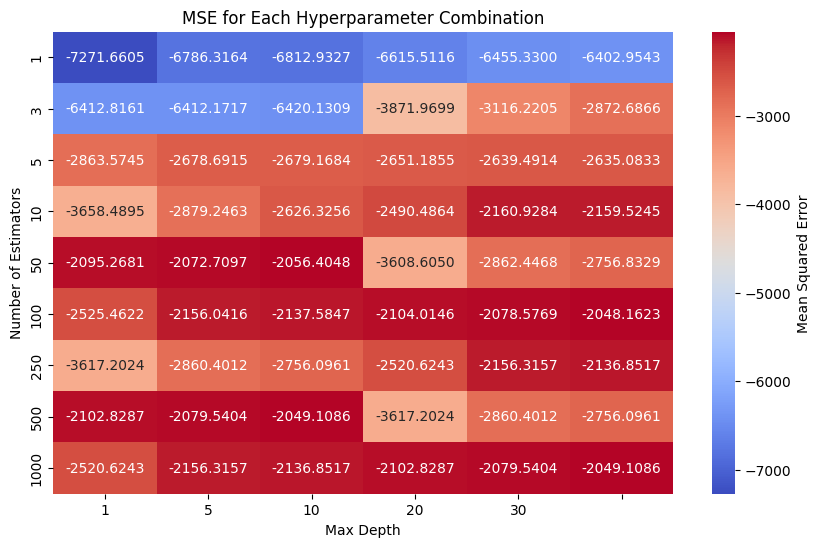
\includegraphics[width=\textwidth]{./images/rfr_mse.jpg}
    \caption{Heatmap of MSE error scores}
\end{figure}
\end{minipage}
\begin{minipage}{0.49\textwidth} 
\begin{figure}[H]
    \centering
    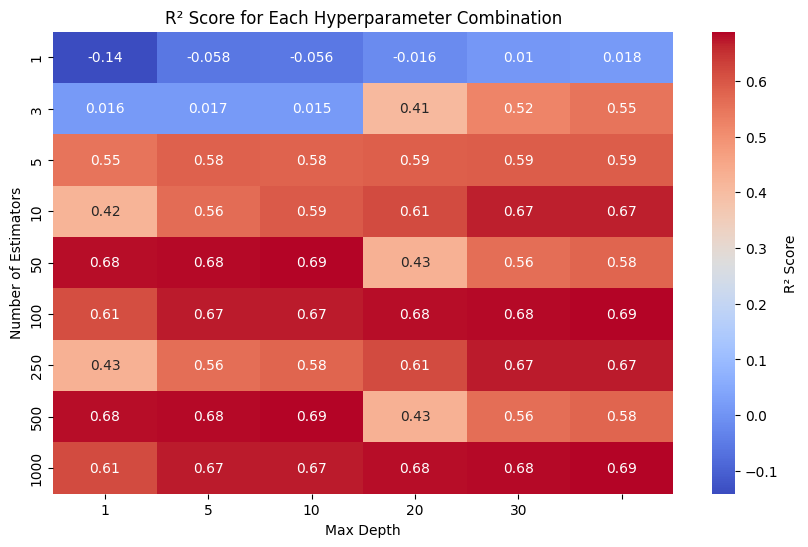
\includegraphics[width=\textwidth]{./images/rfr_r2.jpg}
    \caption{Heatmap of $R^2$ error scores}
\end{figure}
\end{minipage}

As can be seen from the above heatmaps, the best error scores I managed to achieve with hyperparameter tuning were a MSE of approximately -2049 and a corresponding $R^2$ of 0.69, significantly lower than the scores achieved with the default hyperparameter values, achieved with a \mintinline{python}{max_depth} of \mintinline{python}{None} and a \mintinline{python}{n_estimators} of 100.
In this sense, the hyperparameter tuning can be considered a failure as it did not succeed in increasing the accuracy beyond the default values.
One possible reason for this is an insufficiently fine-grain search: the optimal results appear in the 50-500 range for the \mintinline{python}{n_estimators} hyperparameter and a search that focused more on this range could potentially have yielded better results.
However, even the 9 $\times$ 6 level of granularity in searching seen here took around 15-20 minutes to run on my hardware, making finer-grain searching difficult and time-consuming.

\subsection{Algorithm 2: Gradient Boosting}

\begin{code}
\begin{minted}[frame=single]{text}
Average Training MSE: -287.2685
Average Testing  MSE: -783.5938

Average Training  R²: 0.9653
Average Testing   R²: 0.9020
\end{minted}
\caption{Average training \& testing MSE \& $R^2$ with default hyperparameters}
\end{code}

Gradient boosting with the default hyperparameters performed slightly worse than random forest, but had less increase in error in the testing data, lending some credence to the idea that the random forest algorithm may have been slightly overfitting the data.
However, the error scores were nonetheless very good.

\noindent
\begin{minipage}{0.49\textwidth} 
\begin{figure}[H]
    \centering
    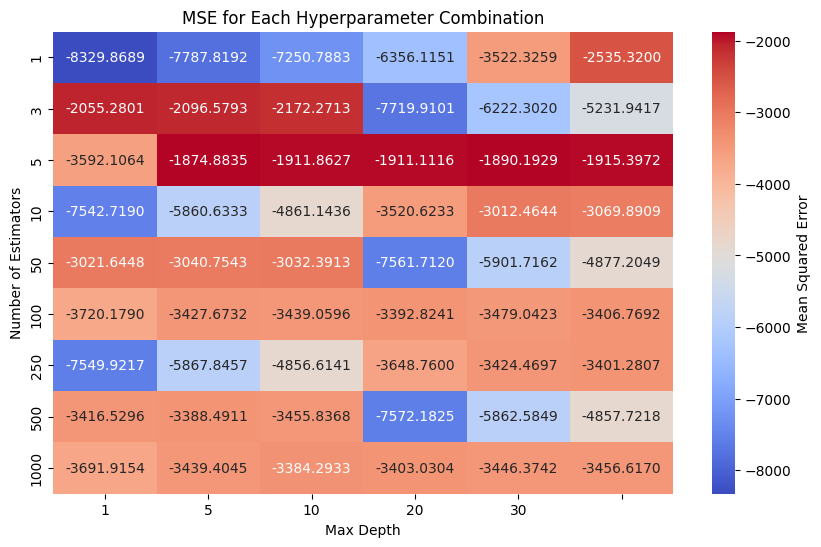
\includegraphics[width=\textwidth]{./images/gbr_mse.jpg}
    \caption{Heatmap of MSE error scores}
\end{figure}
\end{minipage}
\begin{minipage}{0.49\textwidth} 
\begin{figure}[H]
    \centering
    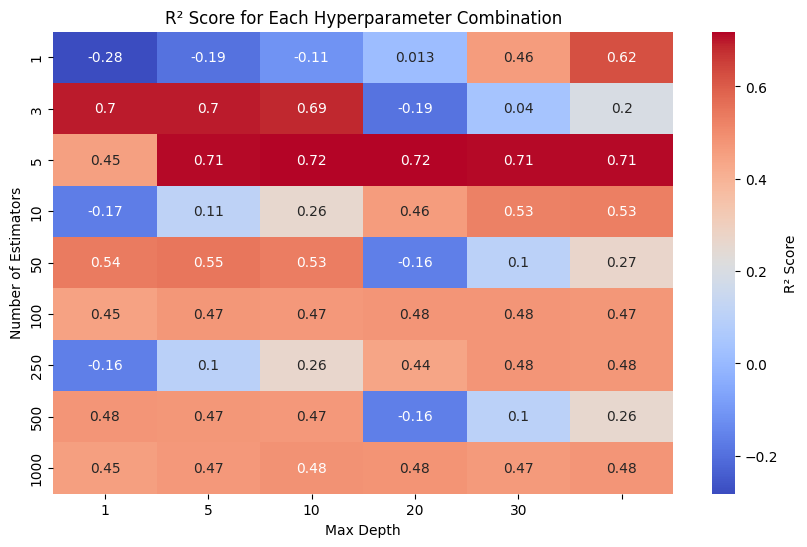
\includegraphics[width=\textwidth]{./images/gbr_r2.jpg}
    \caption{Heatmap of $R^2$ error scores}
\end{figure}
\end{minipage}

As can be seen in the above heatmaps, I again failed to improve on the accuracy achieved by the default hyperparameter values.
Part of this is almost certainly due to the range of values searched through being poor: to maximise comparability with the random forest algorithm I used the same search range, but a glance at the heatmaps shows that it performed very poorly with \mintinline{python}{n_estimator} values past 5.
A better search would likely have focused on a smaller range of \mintinline{python}{n_estimator} values.
The best error scores obtained were a MSE of -1911.116 and a $R^2$ of 0.72, beating the random forest hyperparameter tuning, achieved with a \mintinline{python}{max_depth} of 20 and a \mintinline{python}{n_estimators} of 5.
The much lower \mintinline{python}{n_estimators} of 5 here compared to random forest's 100 serves to illustrate a key difference between the two algorithms: random forest performs well by aggregating many trees covering random, overlapping subsets of the data, so a higher number of trees can increase stability and reduce variance.
The gradient boosting algorithm, on the other hand, makes incremental improvements to the estimators, each one trying to correct the errors of the previous one, allowing it to attain higher accuracy with fewer, more precise trees.

\section{Conclusion}
The key findings are as follows:
\begin{itemize}
    \item   For both algorithms, the default hyperparameters out-performed my attempt at hyperparameter tuning.
            Thus, I can only recommend the default hyperparameter values for both algorithms.
    \item   With the default hyperparameters, \mintinline{python}{RandomForestRegressor} out-performed \mintinline{python}{GradientBoostingRegressor}.
    \item   However, the best hyperparameter tuning results obtained by \mintinline{python}{GradientBoostingRegressor} out-performed the best tuning results obtained by \mintinline{python}{RandomForestRegressor}.
    \item   An exhaustive grid search of 10-fold cross-validated models is highly computationally intensive, and thus very time-consuming.
            Therefore, choosing a small but appropriate range of potential hyperparameter values is key to success if hardware or computation time is limited.
\end{itemize}



\nocite{*}
\printbibliography
\end{document}
